\chapter{Generative Adversarial Networks - Améliorations}


\section{Apprentissage par Mini-Batch}
\subsection{Principe}
L'apprentissage par Batch consiste à apprendre sur l'ensemble du batch d'apprentissage avant de mettre à jour chaque réseau, et de réitérer l'apprentissage à chaque itération sur l'ensemble du batch d'apprentissage.

On calcule successivement la rétropropagation pour chaque image, on somme l'erreur sur l'ensemble des images et on applique la mise à jour du réseau avec la somme des erreurs. On obtient donc une moyenne des directions de propagation afin d'effectuer la mise à jour.

Certaines bases d'apprentissage étant très grandes - soixante mille avec MNIST par exemple -, on va préférer à l'apprentissage par batch, l'apprentissage par Mini-batch. 
On sélectionne aléatoirement parmi la base d'apprentissage un nombre 
\subsection{Implémentation}
Dans le cas de MNIST, les chiffres du début de la bdd étant plus simple, nous avons afin d'obtenir de meilleurs résultats parfois effectué une sélection aléatoire sur uniquement une première partie des 60000 images d'apprentissage (cf argument \textit{labelTrainSize}) et des 10000 images de tests (cf argument \textit{labelTestSize}.
\subsection{Résultats}
Notre équipe a obtenu des résultats peu convaincants, et très différents des résultats du groupe Salamandre 


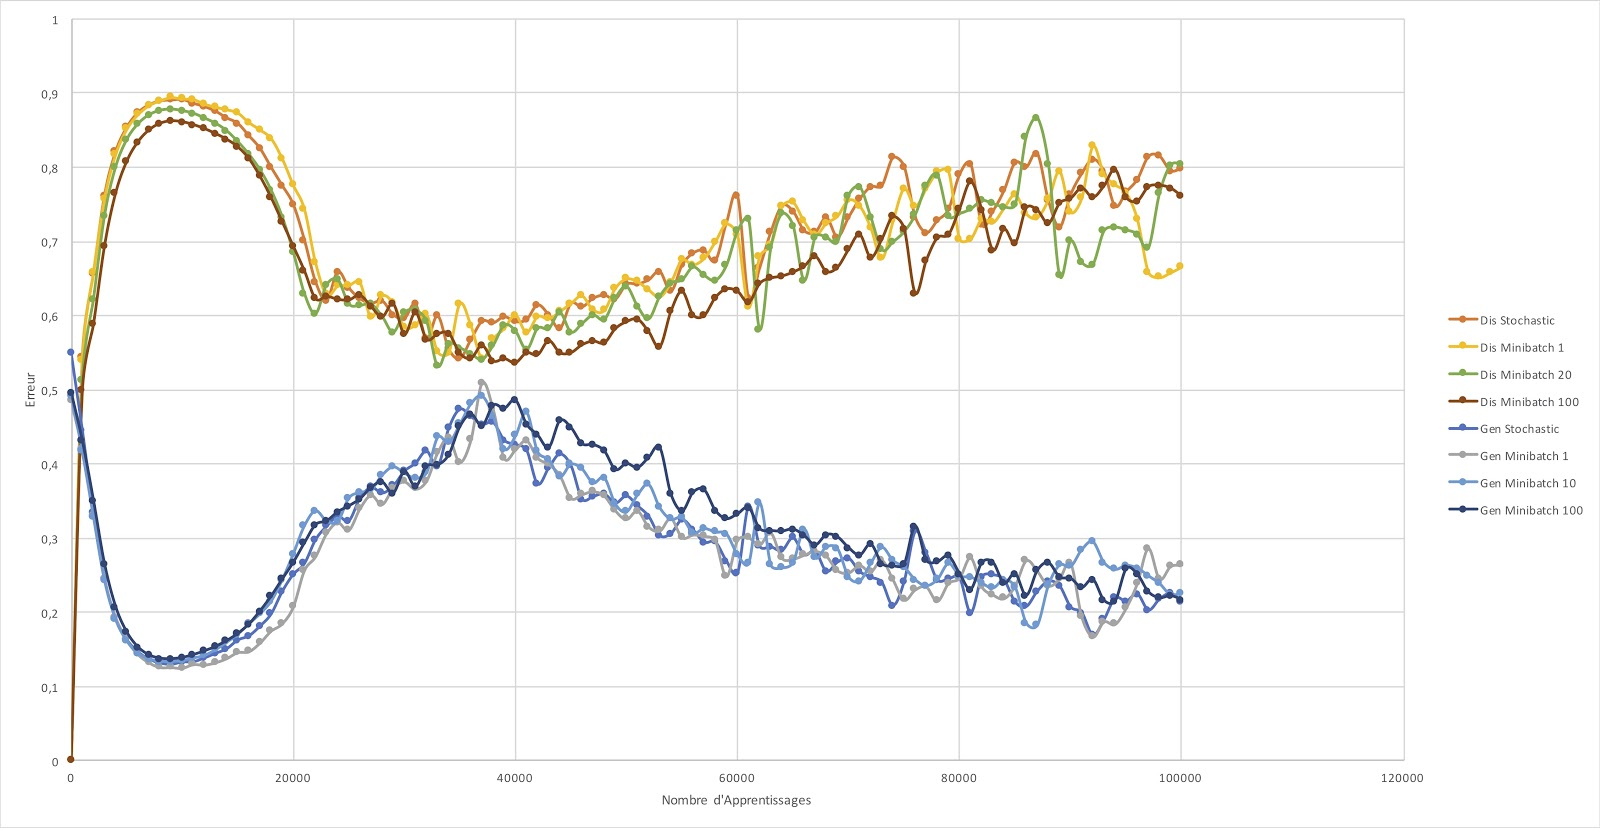
\includegraphics[width=0.5\textwidth]{images/08-gan_ameliorations_resultats_1.jpg}


cf présentation du 15-02-18


\section{Pas adaptatif}
\subsection{RMSprop}

\section{Réseaux à convolution}



